 \documentclass{article}
    \usepackage{amsmath}
    \usepackage[utf8]{inputenc}
    \usepackage[english]{babel}
    \usepackage{color}
    \usepackage{graphicx}
    \usepackage{enumitem}
    % \usepackage[T1]{fontenc}
    \usepackage{geometry}
    
    \usepackage[familydefault,light]{Chivo} 
    \usepackage[T1]{fontenc}
    
    \setlength{\parindent}{4em}
    \setlength{\parskip}{1em}
\renewcommand{\baselinestretch}{1.5}
    \usepackage{graphicx}
    
    \title{COL 783 \\ Assignment 1}
    \author{Rajbir Malik \\ 2017CS10416}
    
    \begin{document}
    
    \maketitle
    
    \begin{center}
    \Large{\underline{\textbf{Tone Mapping HDR Images}}}
    \end{center}
    \subsection*{Overview}
    In this assignment, we were asked to understand and try various tone mapping methods/algorithms on \texttt{HDR} images. We progressively managed to get a better map by first trying fixing the \textbf{linear scale}, then \textbf{logarithmic scale} and eventually an algorithm in general use. I chose to implement {\small \textit{Reinhard et al., “Photographic Tone Reproduction for Digital Images”}}.
    The assignment was divided in 3 different sections, each of which are discussed separately, later.
    
    \pagebreak
    \subsection*{Linear and Logarithmic Rescaling}
    Linear scaling was used to map the complete range (Luminance) of the HDR image between different (min - max) values. Following were the results produced with different scales,
    \begin{itemize}
        \item \textit{Scaling, with large range} : Pixels with large values lose value in the image.
        \item \textit{Scaling, with small range} : Pixels with small values lose value in the image.
        \item \textit{Scaling, with range in between} : Somewhat decent, still this time many of lower and higher range pixels lose value in the image.
    \end{itemize}
    \begin{figure}[!htb]
    \minipage{0.32\textwidth}
      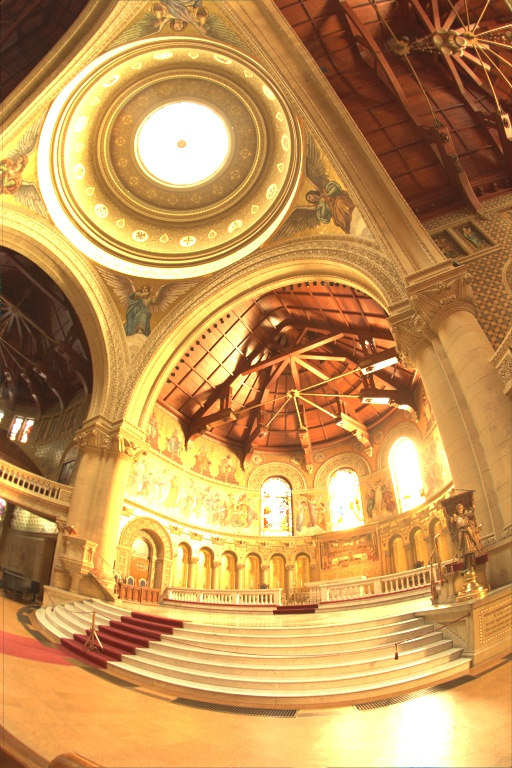
\includegraphics[scale=.27]{./data/1/linscl/mn.jpg}
      \caption{Scaling, with large range}
    \endminipage\hfill
    \minipage{0.32\textwidth}
      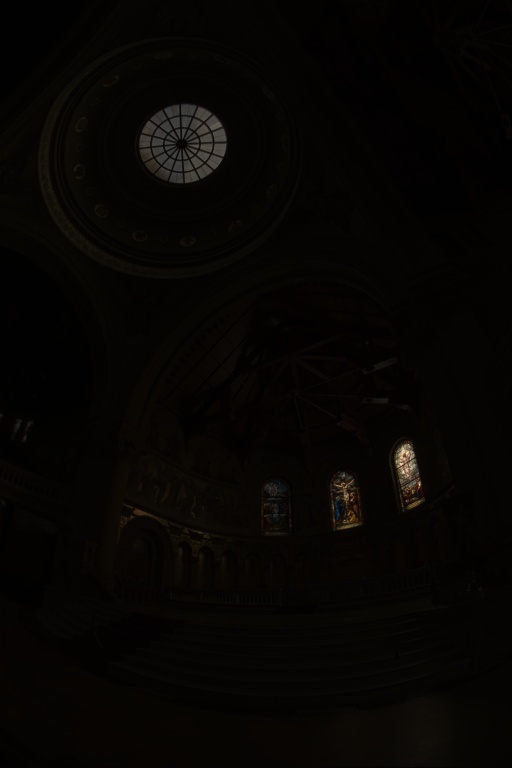
\includegraphics[scale=.27]{./data/1/linscl/mx.jpg}
      \caption{Scaling, with small range}
    \endminipage\hfill
    \minipage{0.32\textwidth}%
      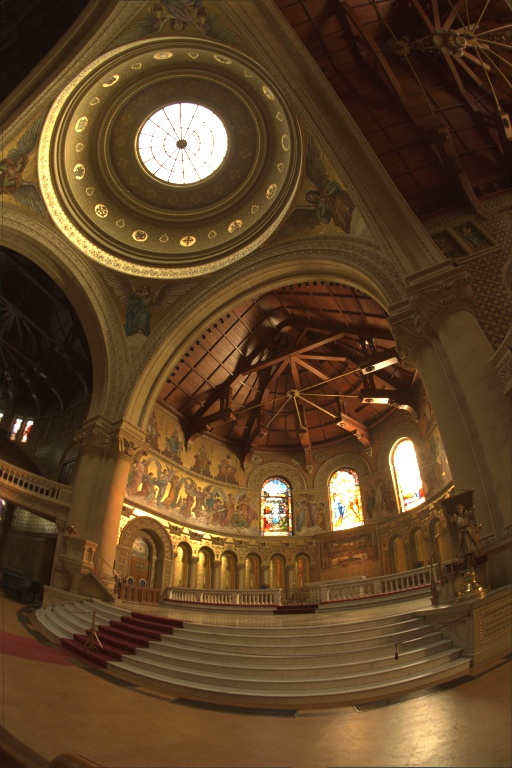
\includegraphics[scale=.27]{./data/1/linscl/md.jpg}
      \caption{Scaling, with range in between}
    \endminipage
    \end{figure}
    \pagebreak
    Logarithmic scaling was implemented by processing the \texttt{log(luminance)}. It had much better results than the linear scaling as it lead to non-linear map which allowed accommodation of closer pixels. I tried in different bases, and the results are as followed,
    \begin{itemize}
        \item \texttt{Base:10} with scaling \texttt{0.1-2.1} (and thus linear scale is 1:100)
        \item \texttt{Base:3} with scaling \texttt{1-6} (and thus linear scale is 1:243)
    \end{itemize}
    
    \begin{figure}[!htb]
    \minipage{0.32\textwidth}
      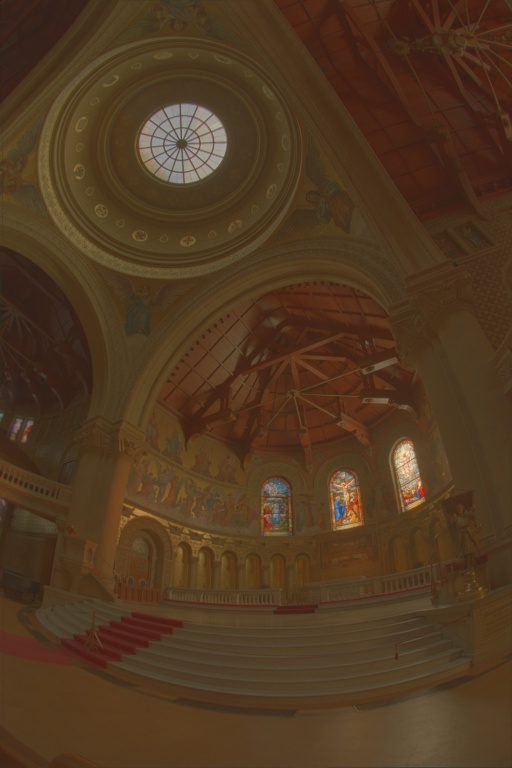
\includegraphics[scale=.4]{./data/1/lgscl/b10.jpg}
      \caption{Base 10}
    \endminipage\hfill
    \minipage{0.32\textwidth}
      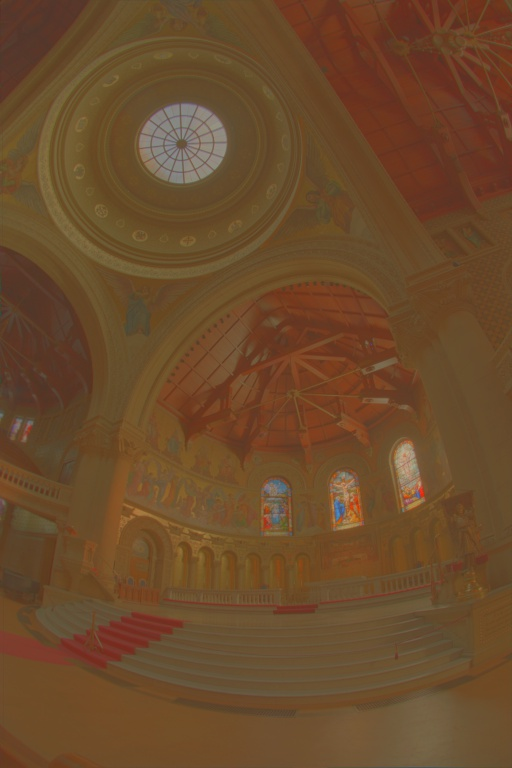
\includegraphics[scale=.4]{./data/1/lgscl/b3.jpg}
      \caption{Base 3}
    \endminipage\hfill
    \end{figure}
    
    \\
    Concluding, the images produced by \texttt{log-luminance} rescaling are much better and comprehensive. We shall now pursue improving these images in the next section.
    
    \pagebreak
    \subsection*{Detail Enhancement}
    In this section we apply series of image enhancement techniques to improve the features of the image previously acquired.
    First the image was enhanced in the linear-luminance domain. Following steps were carried out, \\
    \begin{figure}[!htb]
    \minipage{0.32\textwidth}
      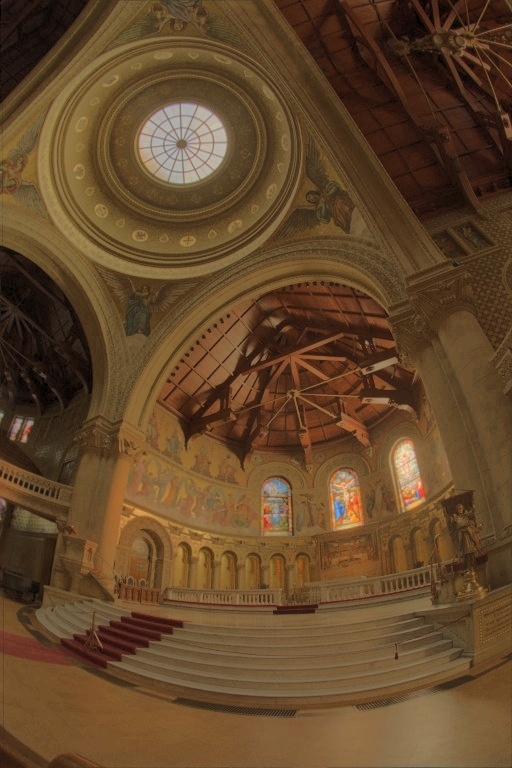
\includegraphics[scale=.27]{./data/2/ln/s1.jpg}
      \caption{Histogram Eq.}
    \endminipage\hfill
    \minipage{0.32\textwidth}
      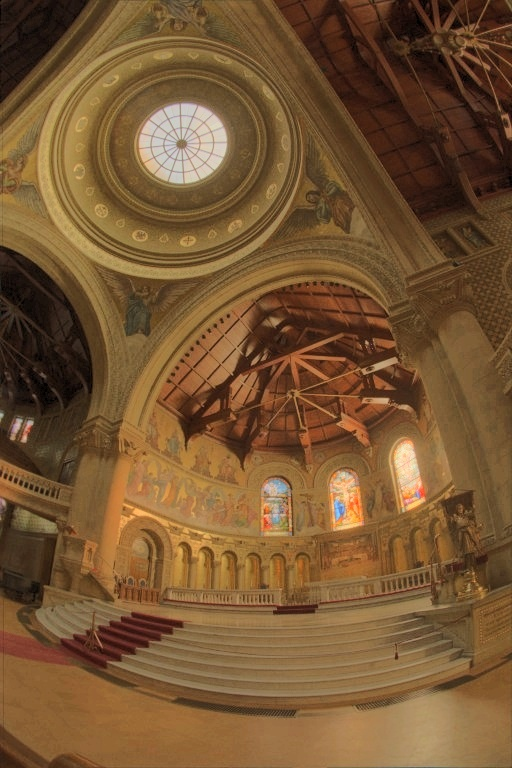
\includegraphics[scale=.27]{./data/2/ln/s2.jpg}
      \caption{Gamma Correction}
    \endminipage\hfill
    \minipage{0.32\textwidth}%
      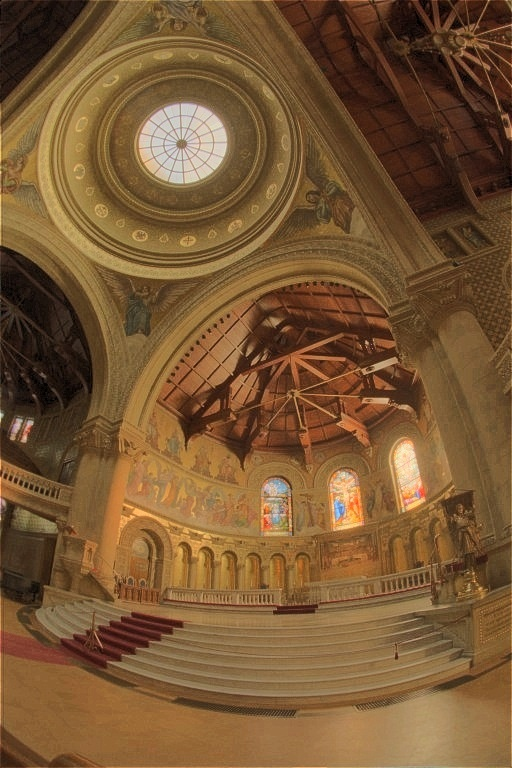
\includegraphics[scale=.27]{./data/2/ln/s3.jpg}
      \caption{Unsharp Masking}
    \endminipage
    \end{figure}

    \pagebreak
    Second the image was enhanced in the log-luminance domain. Following steps were carried out, \\
    \begin{figure}[!htb]
    \minipage{0.32\textwidth}
      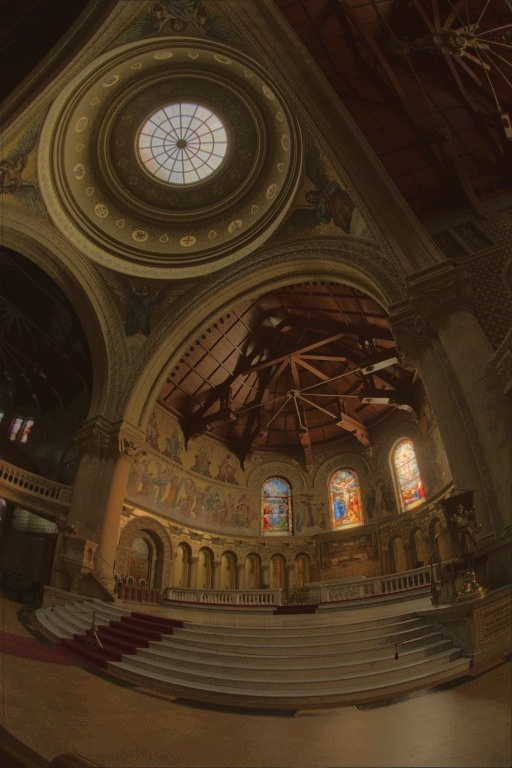
\includegraphics[scale=.27]{./data/2/lg/s1.jpg}
      \caption{Histogram Eq.}
    \endminipage\hfill
    \minipage{0.32\textwidth}
      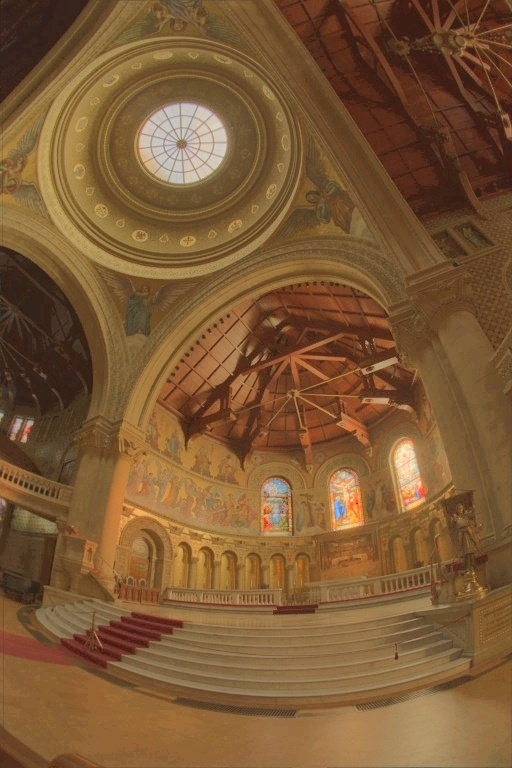
\includegraphics[scale=.27]{./data/2/lg/s2.jpg}
      \caption{Gamma Correction}
    \endminipage\hfill
    \minipage{0.32\textwidth}%
      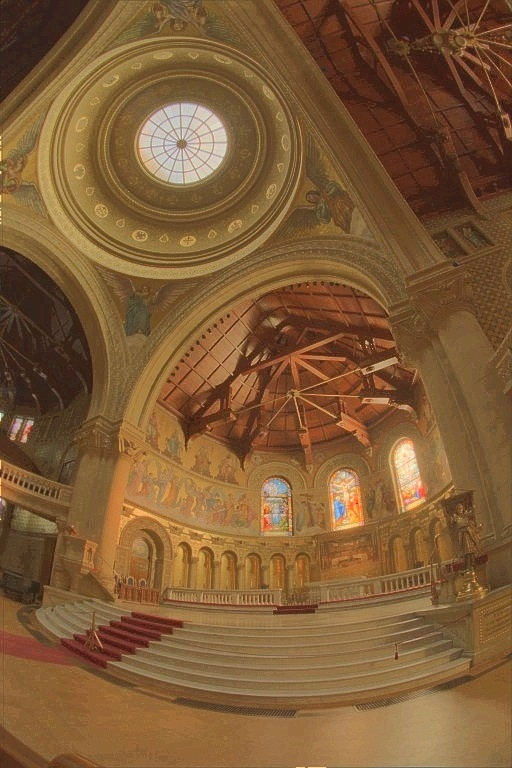
\includegraphics[scale=.27]{./data/2/lg/s3.jpg}
      \caption{Unsharp Masking}
    \endminipage
    \end{figure}
    \\
    Concluding, there is much difference b/w the final images produced except for that log-domain maintains chromaticity better. Also, directly working with RGB values is not logical as there correlation to produce a color is non-zero, and thus any unsynced changes would lead to loss of the original color.
    
    \pagebreak
    
    \subsection*{Tone Mapping Algorithm}
    In this section, I focused on implementing the \textbf{Reinhard Tone Map} and applied on a set of images. The original images produced, were processed to give promising mappings, shown below.
    \begin{center}
        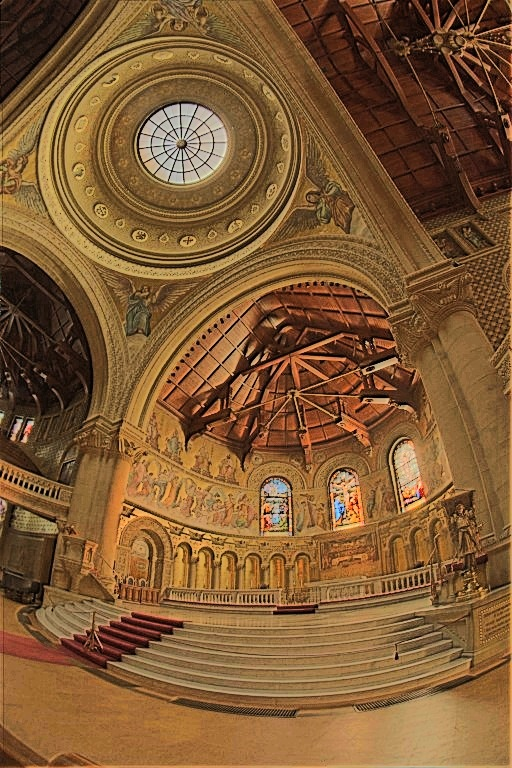
\includegraphics[scale=.27]{./data/3/fnl.jpg}
    \end{center}
    Also, following was the general variation in the deciding s parameter.
    \begin{center}
        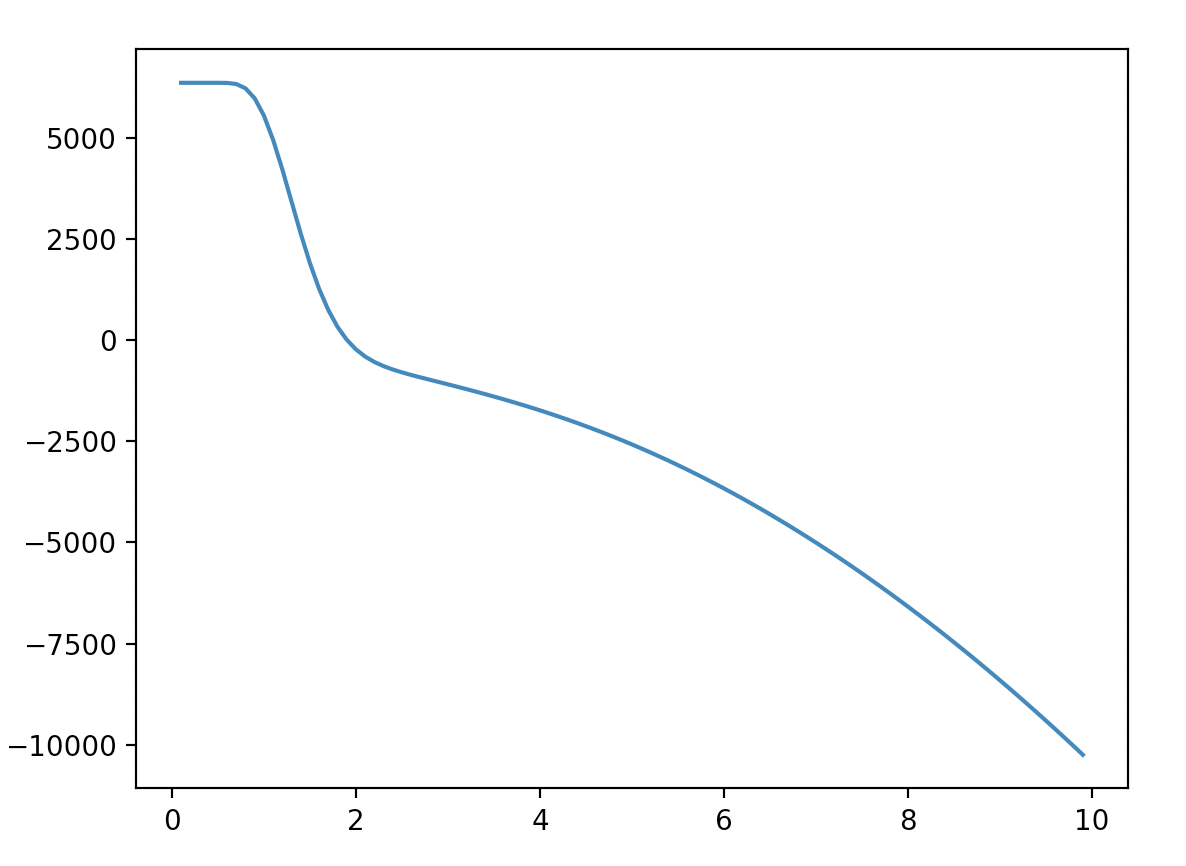
\includegraphics[scale=.27]{./data/3/plot.png}
    \end{center}
    \pagebreak
    Also, following are how images vary if different parameters are set.
    \begin{figure}[!htb]
    \minipage{0.32\textwidth}
      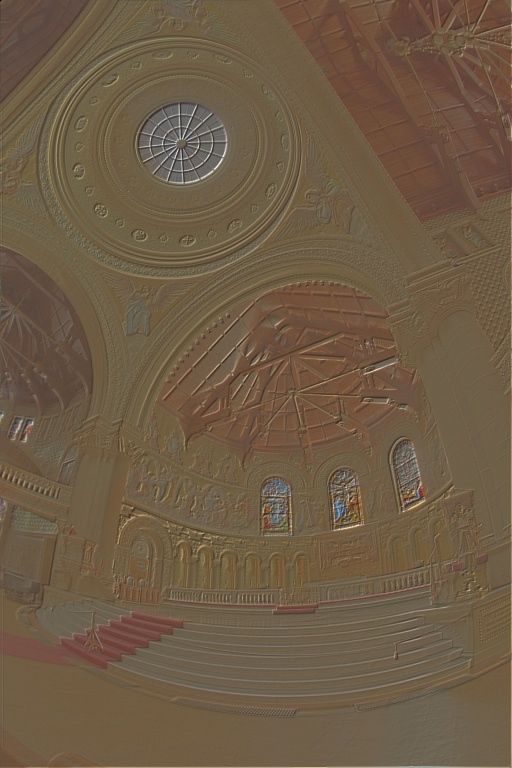
\includegraphics[scale=.27]{./data/3/svar/s1.jpg}
      \caption{s = 0.1}
    \endminipage\hfill
    \minipage{0.32\textwidth}
      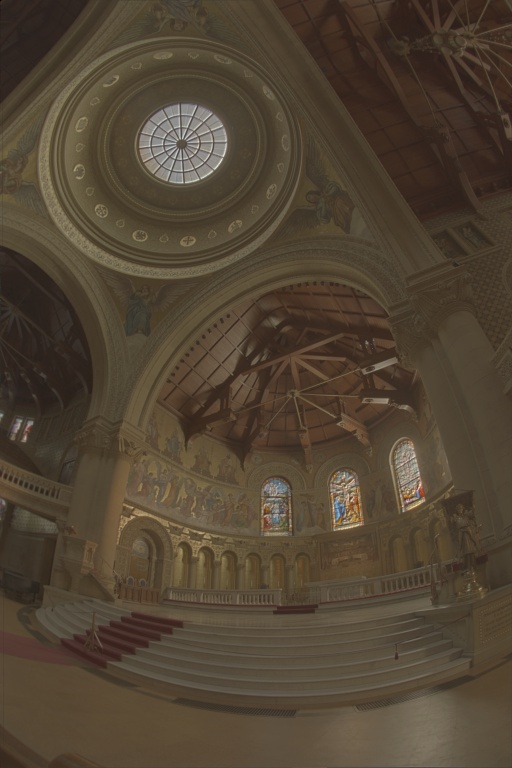
\includegraphics[scale=.27]{./data/3/svar/s2.jpg}
      \caption{s = 2.1 (Optimal)}
    \endminipage\hfill
    \minipage{0.32\textwidth}%
      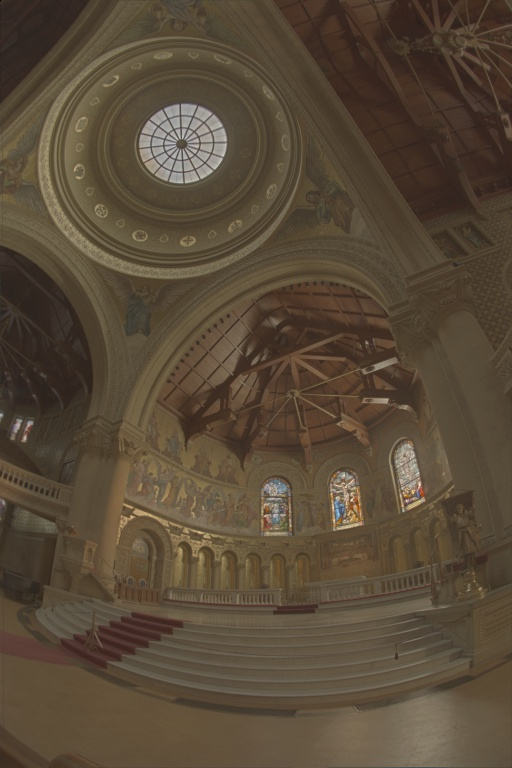
\includegraphics[scale=.27]{./data/3/svar/s3.jpg}
      \caption{s = 9.9}
    \endminipage
    \end{figure}
    \begin{figure}[!htb]
    \minipage{0.32\textwidth}
      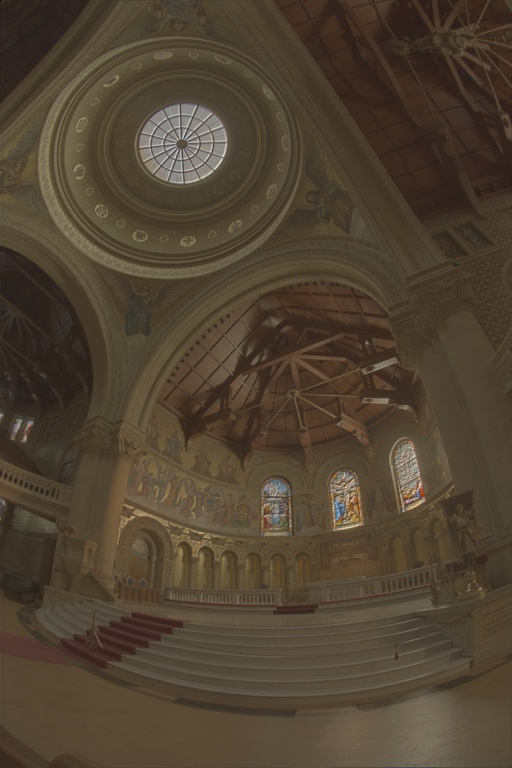
\includegraphics[scale=.27]{./data/3/avar/3_6.jpg}
      \caption{key = .36}
    \endminipage\hfill
    \minipage{0.32\textwidth}
      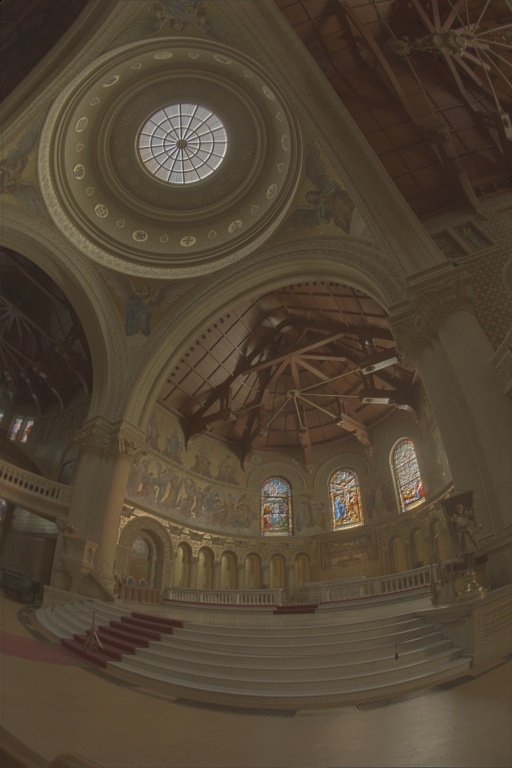
\includegraphics[scale=.27]{./data/3/avar/4_5.jpg}
      \caption{key = .45}
    \endminipage\hfill
    \minipage{0.32\textwidth}%
      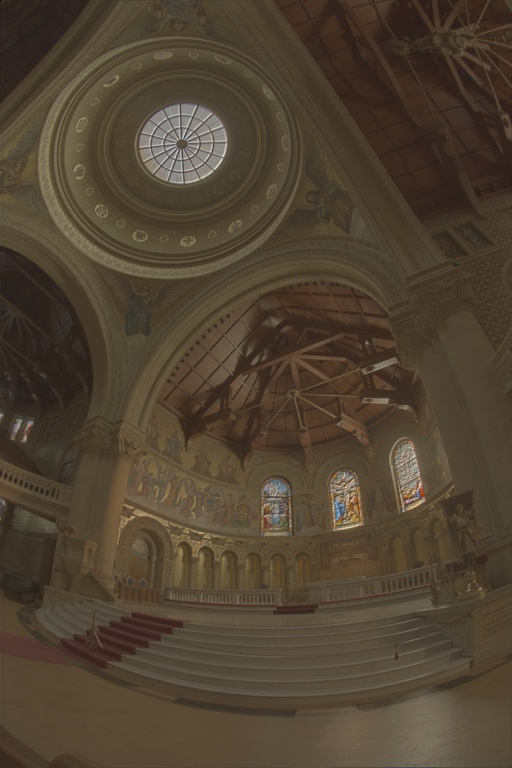
\includegraphics[scale=.27]{./data/3/avar/7_2.jpg}
      \caption{key = .72}
    \endminipage
    \end{figure}
    
\end{document}